\documentclass{article}

\usepackage{tikz}
\usetikzlibrary{calc}


\begin{document}\begin{figure}
   \tikzset{
      tick/.style = {black, very thick}
    }

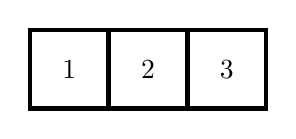
\begin{tikzpicture} % boxlength=1%ZEILE NR. 0 (von unten)

%ELEMENT IN SPALTE NR. 0 (von links)
\draw [ultra thick] (0,0) rectangle (1,1);
\node at ($(0.5,0.5)$) {$1$};

%ELEMENT IN SPALTE NR. 1 (von links)
\draw [ultra thick] (1,0) rectangle (2,1);
\node at ($(1.5,0.5)$) {$2$};

%ELEMENT IN SPALTE NR. 2 (von links)
\draw [ultra thick] (2,0) rectangle (3,1);
\node at ($(2.5,0.5)$) {$3$};






\end{tikzpicture}
\end{figure}
\end{document}